\section{Tīkla testi}
Šajā testā tiek pārbaudīta vadības sistēma no operatora datora līdz mikrokontrolieram ar skripta palīdzību, kas rakstīts Python priekš Windows OS. Tests tika veikts izolētā tīklā, kur atradās tikai divas ierīces: operātora dators un mikrokontrolieris ar visu X-joslas sistēmu.
\begin{figure}[H]
	\centering
    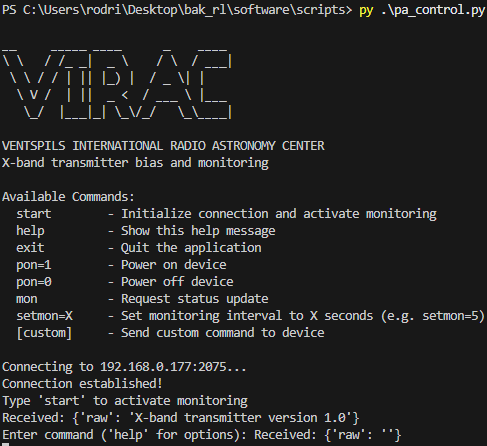
\includegraphics[width=0.9\textwidth]{pictures/script_start.png}\hspace{1cm}
    \caption{Klienta konfigurēšana lokālajā tīklā}
\end{figure}
Tests sākās ar skripta uzsākšanu. Terminālī redzams logo, palīgrinda un to, ka veiksmīgi ir pieslēdzies pie TCP servera, kurš uzreiz pēc pieslēgšanās atsūta savu nosaukumu un versiju. Tad lietotājam tiek sniegta informācija par komandu, kura uzsāk monitorēšanu un darba punkta iestatīšanu. Pēc tā tiek aicināts ievadīt komandu.
\begin{figure}[H]
	\centering
    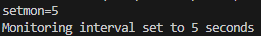
\includegraphics[width=0.9\textwidth]{pictures/script_monchange.png}\hspace{1cm}
    \caption{Monitorēšanas cikla aizkaves maiņa}
\end{figure}
Redzams monitorēšanas intervāla iestatīšanu no noklusētās vērtības 30 sec uz 5 sekundēm.
\begin{figure}[H]
	\centering
    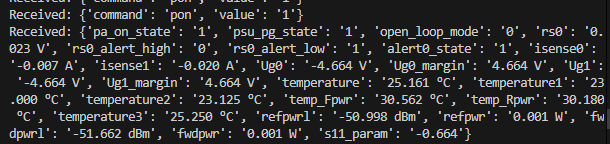
\includegraphics[width=0.9\textwidth]{pictures/script_system_start .png}\hspace{1cm}
    \caption{Darba punkta iestatīšana un telemetrijas virkne}
\end{figure}
Tad tika uzsākta sistēmas darbība ar komandu "start", kur var redzēt, ka tika nosūtīta komanda pon=1 un saņemta atbilde no mikrokontroliera pon=1, kas liecina par to, ka komanda tika saņemta un veiksmīgi apstrādāta. Pēc kā seko monitorēšanas telemetrijas ik pēc 5 sekundēm.
\begin{figure}[H]
	\centering
    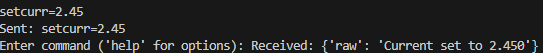
\includegraphics[width=0.9\textwidth]{pictures/script_setcurr.png}\hspace{1cm}
    \caption{Darba punkta noteces strāvas iestatīšana}
\end{figure}
\begin{figure}[H]
Tad tiek iestatīts cita darba punkta strāva no 3 A uz 2.45 A, kur mikrokontrolieris arī deva atbildi, ka tā tika veiksmīgi uzstādīta.
	\centering
    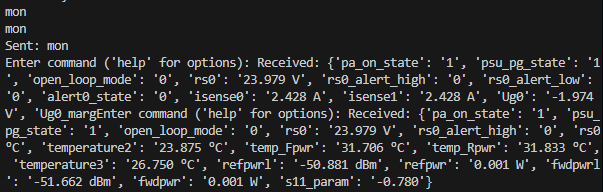
\includegraphics[width=0.9\textwidth]{pictures/script_setcurr_tel.png}\hspace{1cm}
    \caption{Strāvas maiņas telemetrijas virkne}
\end{figure}
Tad var redzēt, ka telemetrijas virknē ir aizvara spriegums cits un noteces strāva 2.426 A.
\begin{figure}[H]
	\centering
    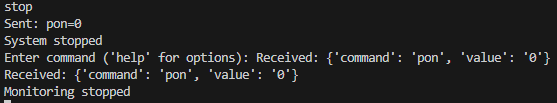
\includegraphics[width=0.9\textwidth]{pictures/script_system_stop.png}\hspace{1cm}
    \caption{Darba punkta atiestatīšana}
\end{figure}
Aktīvu sistēmu var deaktivizēt ar komandas nosūtīšanu "stop", kas uzreiz uz mikrokontrolieri nosūta komandu pon=0 un izbeidz monitorēšanas pavedienu.
\begin{figure}[H]
	\centering
    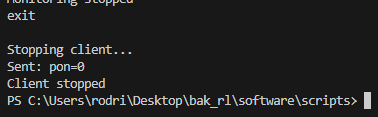
\includegraphics[width=0.9\textwidth]{pictures/script_exit.png}\hspace{1cm}
    \caption{Skripta izslēgšana}
\end{figure}
Ar exit vai ctrl+c var izbeigt skripta darbību, kur tiek aizsūtīta komanda pon=0, lai izslēgtu sistēmu, ja tā bija aktīva, un atvienojas no servera, tad izbeidz visu aktīvo pavedienu darbību.

